\section{Methods}
\label{sec:methods}

\subsection{Data}
\label{sec:data}

The model is trained and evaluated on monthly fields spanning January 1981 to June 2024
(522 months), assembled from two reanalyses.

Atmospheric and surface variables are taken from ERA5 \citep{Hersbach2020}, monthly means of
daily means on the native $0.25\dgr$ grid: sea surface temperature (SST), the 10\,m zonal and
meridional wind components (U10, V10), mean sea-level pressure (MSL), total column
vertically-integrated water vapour (TCWV), total cloud cover (TCC), top-of-atmosphere net
long-wave radiation flux, and the surface latent heat, sensible heat, and total precipitation
fluxes.

Subsurface ocean variables are taken from SODA4 (version 4.15.2)
\citep{Chepurin2025}, monthly means derived from the five-day product on its native
$0.1\dgr$ eddy-resolving grid: the depth of the $20\dgr$C isotherm (Z20, the thermocline
proxy), sea surface height, and mixed-layer depth defined by the temperature criterion. The
SODA fields are conservatively regridded onto the ERA5 grid before use.

Together these thirteen channels span the coupled system -- the surface temperature the
forecast targets, the subsurface structure that carries its memory, and the atmospheric fields
through which the coupling acts. Note that the SST used is the ERA5 field rather than the
ocean model's own surface temperature, so that the forecast target is defined consistently with
the atmospheric state.

The combined fields are cropped to the tropical Pacific, $20\dgr$S--$20\dgr$N,
$120\dgr$E--$290\dgr$E, giving $161\times681$ points per channel. Each channel is then
standardised by a single scalar mean and standard deviation computed over all months and all
grid points, so that the thirteen enter the reconstruction loss on comparable scales. Land
points, which are missing in the ocean channels, are set to zero after standardisation -- that
is, to exactly the channel mean -- and are retained in the loss, so the network must reproduce
the coastline as well as the fields.

The autoencoder therefore operates on complete fields, including the seasonal cycle and the
spatial mean state, rather than on anomalies. Anomalies are formed later and in the latent
space: for each cross-validation fold a twelve-month latent climatology is computed from the
training months of that fold alone and subtracted, and the same climatology is added back to a
forecast latent state before it is decoded. The Ni\~no 3.4 and warm-water-volume climatologies
are constructed the same way. No climatological information from a held-out period therefore
enters the forecast for that period.

Two derived indices are the quantities the model is ultimately scored on. The Ni\~no 3.4 index
is the SST anomaly averaged over $5\dgr$S--$5\dgr$N, $170\dgr$W--$120\dgr$W. Warm-water volume
(WWV) is the Z20 anomaly averaged over $5\dgr$S--$5\dgr$N, $120\dgr$E--$280\dgr$E; in
recharge-oscillator theory \citep{Jin1997} WWV leads SST and constitutes the subsurface memory
that allows a forecast to extrapolate beyond the current SST anomaly.

\subsection{Architecture}
\label{sec:architecture}

The forecast system has three stages: an encoder that compresses the 13-channel field into a
32-dimensional latent state, a modal operator that advances that state in time, and a decoder
that reconstructs physical fields from a forecast latent state. Encoder and decoder are trained
together as an autoencoder and then frozen; the operator is trained separately against that
frozen representation. Table~\ref{tab:config} collects the configuration of both.

\subsubsection{Encoder}
\label{sec:encoder}

The encoder is a windowed transformer in the Swin family \citep{LiuEtAl2021Swin}, modified in
the geometry of its attention windows.

Each monthly field is first coarse-grained by $4\times4$ average pooling, from the native
$0.25\dgr$ grid to $40\times170$ cells of $1\dgr$. This discards sub-degree structure that a
32-dimensional code could not carry in any case, and reduces the token count sixteenfold. The
pooled field is padded by replication to $64\times192$ cells -- the smallest extent divisible
by the patch size and by every window dimension used below -- and embedded by a strided
$4\times4$ convolution into a grid of $16\times48=768$ tokens of dimension 96, each token
corresponding to a $4\dgr\times4\dgr$ block. The replicated margin is removed after decoding
and never enters the loss.

Six window-attention blocks follow. The original architecture partitions the token grid into
square windows; here three geometries are used, chosen to match the anisotropy of the tropical
circulation rather than for computational convenience:

\begin{itemize}
  \item $8\times8$ tokens ($32\dgr\times32\dgr$), a locally isotropic window;
  \item $4\times16$ tokens ($16\dgr$ latitude $\times$ $64\dgr$ longitude), zonally elongated
        to match the east--west Walker circulation;
  \item $16\times4$ tokens ($16\dgr$ of longitude by the full depth of the token grid),
        meridionally elongated to match the north--south Hadley circulation.
\end{itemize}

Each geometry partitions the $16\times48$ token grid into exactly twelve windows of 64 tokens,
so the three differ in shape at identical cost in attention. The meridional window is the
limiting case: the token grid is sixteen rows deep, so a single $16\times4$ window covers every
row, and each token within a $16\dgr$-wide longitude sector attends to the whole
$20\dgr$S--$20\dgr$N band at once.

Each geometry appears twice, once with the window grid aligned to the domain and once displaced
by half a window -- shifts of $(4,4)$, $(2,8)$ and $(8,2)$ tokens respectively -- which is the
mechanism by which windowed attention propagates information across window boundaries. The
displaced partition is implemented as a cyclic roll with the accompanying attention mask, so
that tokens carried from one edge of the domain to the other are prevented from attending to
one another: the domain is a bounded sector of the Pacific, not a periodic channel, and the
mask is what keeps it so.

Attention is multi-head with four heads at dimension 96, and each block is a pre-norm residual
attention followed by a pre-norm two-layer MLP of expansion factor four. There is no relative
position bias and no additive positional encoding. Position therefore enters the representation
only through the convolutional patch embedding, which is spatially local, and through the
window partition itself; the model is told where a token lies only by which window it falls
into, which is the sense in which the choice of window geometry is a modelling assumption about
the circulation rather than an implementation detail.

The 768 token features are reduced to the 32-dimensional state by a learned spatial weighting,
rather than by global average pooling or by a summary token,
\[
z \;=\; \sum_{p=1}^{768} w_p \odot h_p, \qquad w_p \in \mathbb{R}^{32},
\]
where $h_p$ is the feature at token $p$ after a linear projection from 96 to 32 channels and
$\odot$ denotes the elementwise product. Each of the 32 latent coordinates thus carries its own
768-element weight map over the domain, $24{,}576$ parameters in all. The maps are initialised
uniformly at $1/768$, so that at the start of training $z$ is exactly the domain average of the
token features, and each coordinate acquires a distinct spatial footprint only as training
proceeds.

\subsubsection{Decoder}
\label{sec:decoder}

The decoder inverts this, in a form that is deliberately transparent at its first stage. A
latent vector $z\in\mathbb{R}^{32}$ is expanded against a learned per-token basis
$\Phi\in\mathbb{R}^{768\times32}$ and a learned per-token offset $C$, and the result is mapped
back to the 96-dimensional token space by a linear layer $W$:
\[
\tilde h_p \;=\; W\bigl(z \odot \Phi_p + C_p\bigr)
          \;=\; \sum_{d=1}^{32} z_d\,\Phi_{pd}\,W_{:,d} \;+\; \bigl(WC_p + b\bigr).
\]
The reconstructed token field is therefore exactly affine in the latent state: thirty-two fixed
spatial patterns, one per latent coordinate, superposed on a learned climatological field. This
is the structure of an empirical orthogonal function expansion, with the difference that the
patterns are learned jointly with the encoder instead of being eigenvectors of a covariance
matrix, and it is what makes it meaningful to speak of the spatial footprint $\Phi_d$ of an
individual latent coordinate -- the property used in Sec.~\ref{sec:latent-coords}.

The affine stage is followed by six window-attention blocks in the mirror of the encoder's
order, a transposed $4\times4$ convolution back to thirteen channels on the $64\times192$
pooled grid, removal of the replicated margin, and bilinear resampling to $161\times681$. Those
later stages are not linear in $z$, so although each coordinate has a well-defined footprint at
the token level, the complete map from latent state to physical field is nonlinear. This has
one practical consequence used throughout the paper: the blend of Sec.~\ref{sec:blend} is
applied to decoded indices and not to latent states, because decoding does not commute with a
linear combination of latent vectors.

\subsubsection{Resolution of the representation}
\label{sec:compression}

Thirty-two numbers cannot hold a $13\times161\times681$ field, and the architecture determines
the character of what is lost rather than leaving it incidental. Average pooling by four
followed by four-cell patches means that no structure finer than a $4\dgr$ token is
represented; the bilinear resampling at the end restores the grid but not the information. The
representation is therefore a low-pass filter with a known cut-off, not a uniform degradation
of the field, and results obtained through it are statements about the large-scale field. The
fidelity this yields as a function of averaging scale, and the consequence that both indices
the forecast is scored on survive the round trip above $0.99$, are measured in
Sec.~\ref{sec:ae-fidelity}.

\subsubsection{Representation-learning objective}
\label{sec:ae-loss}

The autoencoder is trained on reconstruction with two penalties applied to the latent code:
\[
\mathcal{L}_{\mathrm{AE}} \;=\;
\underbrace{\big\lVert X - \tilde{X}\big\rVert^2_{\mathrm{MSE}}}_{\text{reconstruction}}
\;+\; \lambda_{\mathrm{dec}} \sum_{i\neq j} \big[\mathrm{Corr}(z)\big]_{ij}^{2}
\;+\; \lambda_{2}\,\mathbb{E}\!\left[\lVert z\rVert^2\right],
\]
with $\lambda_{\mathrm{dec}}=10^{-4}$ and $\lambda_{2}=10^{-3}$. The reconstruction term is a
mean squared error over all thirteen channels and all $161\times681$ points in standardised
units, so that every channel contributes on an equal footing by construction.

$\mathrm{Corr}(z)$ is the $32\times32$ correlation matrix of the latent code computed across
the minibatch after standardising each coordinate, and the second term penalises the sum of its
squared off-diagonal entries. Because the minibatch holds 32 samples and the latent dimension
is also 32, that correlation matrix is a noisy estimate: the penalty acts as a stochastic
regulariser accumulated over training rather than as a constraint enforced at any single step.
The decorrelation actually achieved is therefore verified after the fact rather than assumed,
by computing the participation ratio of the latent covariance over the whole record
(Sec.~\ref{sec:latent-coords}). The third term bounds the magnitude of the code, preventing the
network from inflating latent variance to carry structure the decoder cannot use.

This objective is the reason the latent space is close to isotropic rather than an ordered,
variance-ranked hierarchy: it explicitly removes the incentive to concentrate variance in a
few leading directions. The consequence -- a participation ratio of 28.9 of 32, and the
resulting fact that ranking coordinates by variance alone is uninformative -- is measured in
Sec.~\ref{sec:latent-coords}, and is a property of this loss rather than an emergent finding.

The encoder--decoder pair is trained on the full 1981--2024 record as an unsupervised
representation; it is not fit to any forecasting objective, and both the model and the
benchmark (Sec.~\ref{sec:blend}) decode through the same frozen decoder, so any comparison
between them is unaffected by encoder bias.

\subsubsection{Modal operator}
\label{sec:operator}

The latent state is advanced by an operator with a fixed and deliberately restrictive
structure. Its input is a phase vector assembled from a nine-month history -- the current
state, its three-month and eight-month differences, and a convolutional summary of the window,
\[
\phi \;=\; \bigl[\,z(t),\ \Delta_3 z,\ \Delta_8 z,\ \mathrm{conv}\,\bigr] \in \mathbb{R}^{128},
\]
where the last block is produced by a one-dimensional convolution of kernel length nine applied
across the 32 latent channels, so that it mixes over lag and over coordinates at once. The
state handed to the propagator is a learned residual correction of the current state,
$z_0 = z(t) + \mathrm{MLP}_{\phi}(\phi)$, whose output layer is zero-initialised so that
$z_0 = z(t)$ exactly at the start of training.

The operator's time-invariant part is a modal generator,
\[
L_0 = Q\,\mathrm{blockdiag}(B_1,B_2,B_3,D)\,Q^{\top},
\]
where $Q=\exp(\Omega-\Omega^{\top})$ is orthogonal by construction. Three $2\times2$ blocks
$B_k$ each represent a damped oscillator in rotation-plus-decay form, with angular frequency
$\omega_k$ and damping rate $\sigma_k$. Both are bounded by their parameterisation rather than
learned freely: $\sigma_k = 0.005 + 0.045\,\mathrm{sigmoid}(\cdot)$ per month, so that every
mode is damped and stability is imposed rather than discovered, and $\omega_k$ is confined to
periods between one and ten years. The oscillators are initialised at 2.5, 4.0, and 6.0 years
and at an identical damping of $0.0275\,\mathrm{month}^{-1}$, the midpoint of that bound, so
that any ordering of damping rates recovered after training is acquired rather than assumed.
$D$ is a diagonal block of 26 non-oscillatory decay modes under the same damping bound, giving
the full 32-dimensional state. Both constraints govern how the
learned spectrum of Sec.~\ref{sec:modal-spectrum} may be read, and we return to them in the
Discussion.

The generator is modulated by the calendar to represent ENSO's phase-locking to the seasonal
cycle, giving a Floquet system -- linear, but time-periodic:
\[
L_m = L_0 + \cos\theta_m\,L_c + \sin\theta_m\,L_s, \qquad \theta_m = \frac{2\pi m}{12},
\]
so that twelve monthly propagators $\mathcal{T}_m = \exp(L_m)$, $m=1,\dots,12$, follow from one
shared generator. $L_c = W_c - W_c^{\top}$ and $L_s = W_s - W_s^{\top}$ are skew-symmetric by
construction, which restricts the seasonal term to a rotation of the state: it can redirect
energy between latent directions but cannot add or remove it, so that all growth and decay is
confined to $L_0$.

A forecast initialised in calendar month $m$ is then the ordered product of the propagators for
the months actually traversed,
\[
z_{\mathrm{lin}}(l) \;=\; g(\phi)\; z_0^{\top}\,
\mathcal{T}_{m+1}\mathcal{T}_{m+2}\cdots\mathcal{T}_{m+l}, \qquad l = 1,\dots,24,
\]
where $g(\phi) = 1 + 0.5\tanh(\cdot) \in [0.5,1.5]$ is a bounded, state-dependent scalar gain.
Its pre-activation is batch-normalised without affine parameters, so that $g$ averages one
across a minibatch and redistributes amplitude between forecasts rather than inflating all of
them; its linear layer is zero-initialised, so $g=1$ exactly at the start of training. Because
$g$ is a single positive factor applied to the whole 24-month trajectory, it can change
amplitude but not sign, and cannot by itself introduce El Ni\~no/La Ni\~na asymmetry.

Two further terms are added to this gained linear path. The first is a gated nonlinear
residual, $\gamma\,\mathrm{MLP}(\phi,\theta_m)$, a two-layer network of 64 hidden units taking
the phase vector together with a two-component embedding $(\sin\theta_m,\cos\theta_m)$ of the
initialisation month, and emitting the full $24\times32$ correction at once. The second is a
low-rank direct linear term $W_{\mathrm{out}}(W_{\mathrm{in}}\phi)$, in which $W_{\mathrm{in}}$
projects the phase vector to rank four and $W_{\mathrm{out}}$ expands it to the same
$24\times32$ output; this is the fast, tendency-like path that the observational benchmark also
exploits. The complete forecast is
\[
\hat z(l) \;=\;
\underbrace{g(\phi)\,z_0^{\top}\,\textstyle\prod_{j=1}^{l}\mathcal{T}_{m+j}}
           _{\text{Floquet propagation}}
\;+\; \underbrace{\gamma\,\mathrm{MLP}(\phi,\theta_m)\big|_l
\;+\; W_{\mathrm{out}}(W_{\mathrm{in}}\phi)\big|_l}_{\text{initial-condition corrections}},
\qquad l = 1,\dots,24,
\]
where $|_l$ selects the lead-$l$ block of the $24\times32$ output.

Two properties of this decomposition are worth stating explicitly, because the paper's
interpretability claims rest on them. First, both additive terms are functions of the initial
phase vector alone, and neither is applied recursively; the only part of the forecast that
compounds with lead is the ordered product of monthly propagators, which is precisely the part
whose eigenstructure is reported in Sec.~\ref{sec:modal-spectrum}. Second, every correction is
inert at initialisation: $W_{\mathrm{out}}$, the residual MLP's output layer, the gain's linear
layer and the initial-state correction's output layer are all zero-initialised, and $\gamma$ is
additionally held at exactly zero for the first 40\% of epochs. Training therefore begins from
a pure Floquet propagation of the observed latent state, and each correction is acquired only
insofar as it reduces the loss.

Figure~\ref{fig:workflow} shows the propagated linear path and the gated nonlinear residual,
the two terms that carry the central architectural claims; the initial-state correction, the
gain, and the low-rank direct term are omitted there for legibility but are present in every
trained model.

\begin{table}[t]
\centering
\caption{Configuration of the two trained components, as instantiated. Window sizes are given
in tokens; one token is a $4\dgr\times4\dgr$ block of the pooled grid.}
\label{tab:config}
\small
\begin{tabular}{@{}ll@{}}
\toprule
Setting & Value \\
\midrule
\multicolumn{2}{@{}l}{\textit{Autoencoder}} \\
\quad Input & 13 channels, $161\times681$, $0.25\dgr$ \\
\quad Pooling, patch, tokens & $4\times4$ mean; $4\times4$ patch; $16\times48=768$ tokens, dim 96 \\
\quad Window geometries & $8\!\times\!8$, $4\!\times\!16$, $16\!\times\!4$ tokens; each shifted and unshifted \\
\quad Attention & 4 heads; MLP expansion 4; no positional encoding \\
\quad Latent & 32-D, learned spatial weighting ($24{,}576$ weights) \\
\quad Loss & MSE $+\ 10^{-4}\sum_{i\neq j}\mathrm{Corr}(z)^2_{ij} + 10^{-3}\,\mathbb{E}\lVert z\rVert^2$ \\
\quad Parameters & $1{,}462{,}317$ \\
\midrule
\multicolumn{2}{@{}l}{\textit{Modal operator}} \\
\quad Phase vector & $[z,\Delta_3 z,\Delta_8 z,\mathrm{conv}]$ from a 9-month history, dim 128 \\
\quad Oscillators & 3, initialised at 2.5 / 4.0 / 6.0 yr; periods bounded to 1--10 yr \\
\quad Damping & $0.005$--$0.05$ month$^{-1}$ on all 32 modes, imposed \\
\quad Seasonality & Floquet: 12 monthly propagators from one generator \\
\quad Corrections & gain $\in[0.5,1.5]$; $\gamma$-gated MLP (64 hidden); rank-4 linear \\
\quad Parameters & $79{,}682$ \\
\bottomrule
\end{tabular}
\end{table}

\subsection{Forecast: blending with an observable benchmark}
\label{sec:blend}

The reported forecast is not the operator's raw output. It is a fixed-weight blend of the
hybrid (operator) forecast with an observable-predictor benchmark,
\[
\hat y(l) = \mathrm{benchmark}(l) + \alpha(l)\,\bigl[\mathrm{hybrid}(l) -
\mathrm{benchmark}(l)\bigr], \qquad
\alpha(l) = \begin{cases} 0.25 & l = 1,\dots,18 \\ 0 & l = 19,\dots,24. \end{cases}
\]
The benchmark is a per-fold ordinary least-squares map from four observed predictors at
initialisation -- Ni\~no 3.4, WWV, and their 3-month tendencies -- to the 32-dimensional latent
anomaly at lead $l$. $\alpha$ is a fixed constant, not a fitted parameter: results are flat for
$\alpha\in[0.15,0.40]$, and the lead-18 cutoff is set by where the operator's residual stops
carrying statistically significant information, not by tuning ACC.

The blend is applied to decoded indices rather than to latent states, for the reason given in
Sec.~\ref{sec:decoder}. Because it is linear in $\alpha$, skill and amplitude can be computed
for any value of $\alpha$ without retraining, using only the stored benchmark and raw hybrid
forecasts; this is used in Sec.~\ref{sec:results} to characterise the blend as a quantified
trade rather than a fixed, unexamined choice.

\subsection{Training the operator}
\label{sec:training}

The operator is trained to predict the latent trajectory as a residual on the benchmark: for
each initialisation, the network output is added to the benchmark's latent prediction
(Sec.~\ref{sec:blend}) and the sum is scored. The objective combines four terms, applied both
in latent space and, after decoding, at the two indices the paper reports:
\[
\mathcal{L} \;=\;
\underbrace{\mathcal{L}^{\mathrm{MSE}}_{\mathrm{lat}}
+ \mathcal{L}^{\mathrm{ACC}}_{\mathrm{lat}}}_{\text{latent}}
\;+\; \frac{1}{|S|}\sum_{l\in S}
\Big[\,2\,\mathcal{L}^{\mathrm{MSE}}_{\mathrm{N3.4}}(l)
+ \mathcal{L}^{\mathrm{ACC}}_{\mathrm{N3.4}}(l)
+ 2\,\mathcal{L}^{\mathrm{MSE}}_{\mathrm{WWV}}(l)
+ \mathcal{L}^{\mathrm{ACC}}_{\mathrm{WWV}}(l)\Big].
\]
Here $\mathcal{L}^{\mathrm{ACC}} = 1 - r$, with $r$ the Pearson correlation computed across the
minibatch, so that correlation is optimised directly rather than only through squared error.
The latent MSE term is weighted linearly by lead, from $0.5$ at lead 1 to $3.0$ at lead 24, so
that long leads -- where the forecast is hardest and where an unweighted MSE would contribute
least -- are not dominated by short leads.

The index terms require decoding, which is expensive to apply at all 24 leads for every
minibatch. Instead, $S$ is a random subset of six leads drawn per minibatch without replacement,
with sampling probability increasing linearly with lead over the same $0.5$--$3.0$ range; the
WWV term is normalised by the training-period standard deviation of the WWV anomaly so that the
two indices contribute on comparable scales. Because the decoder is frozen, gradients from
these index terms propagate back through it into the operator without changing the
representation.

Optimisation uses CA-AdamW, a curvature-aware variant of AdamW
\citep{AnEtAl2026}, with learning rate $10^{-3}$, weight decay $10^{-4}$, curvature scale
$\alpha_{\mathrm{base}}=0.1$, and a cosine-annealed schedule decaying to $10^{-4}$; gradients
are clipped to unit norm. Models are trained for 301 epochs at batch size 32. The gate $\gamma$
is held at exactly zero, with its gradient disabled, for the first 40\% of epochs (120 of 301),
then set to $0.05$ and trained, so that the linear operator is fit before any nonlinear
correction becomes available.

The autoencoder is trained separately and beforehand, for 2500 epochs at batch size 32 over the
522-month record (about $42{,}500$ optimisation steps), using CA-AdamW with learning rate
$2\times10^{-3}$, weight decay $10^{-4}$, a warm-up of 50 steps followed by cosine decay to
$5\times10^{-4}$, unit-norm gradient clipping, and mixed-precision arithmetic. It is frozen
thereafter.

\subsection{Validation protocol}
\label{sec:validation}

Skill is assessed by temporal cross-validation over four folds -- 1981--1991, 1991--2002,
2002--2013, 2013--2024 -- with a 24-month buffer removed around each held-out period so that no
verification target overlaps, even partially, with any training window. Ten random seeds are
trained per fold, giving 40 trained models in total; reported skill is the seed ensemble unless
stated otherwise. In total there are 394 verification windows, each a full 24-month forecast,
spanning 42 independent winters.

Three reference forecasts are reported alongside the model: the observable-predictor benchmark
(Sec.~\ref{sec:blend}); persistence, the observed Ni\~no 3.4 anomaly at initialisation held
flat; and climatology (zero anomaly), against which RMSE is normalised in
Sec.~\ref{sec:results} so that a value of 1.0 corresponds exactly to a climatological forecast.

Uncertainty is quantified throughout by a paired year-block bootstrap: the 36 distinct
initialisation years are resampled with replacement as blocks (rather than resampling
individual, overlapping 24-month windows, which are not independent), and the model and
benchmark are recomputed on the same resampled set so that comparisons remain paired. Unless
noted otherwise, this uses 10\,000 draws (seed 0) for the deterministic skill and seasonal
results and 5\,000 draws (seed 0) for the event-discrimination and case-study results. All
reported intervals are 95\%, and significance is stated as $p<0.05$ or as a 95\% confidence
interval excluding zero -- never as a value of $\alpha$, which is reserved exclusively for the
blend weight (Sec.~\ref{sec:notation}).

\begin{figure}[t]
  \centering
  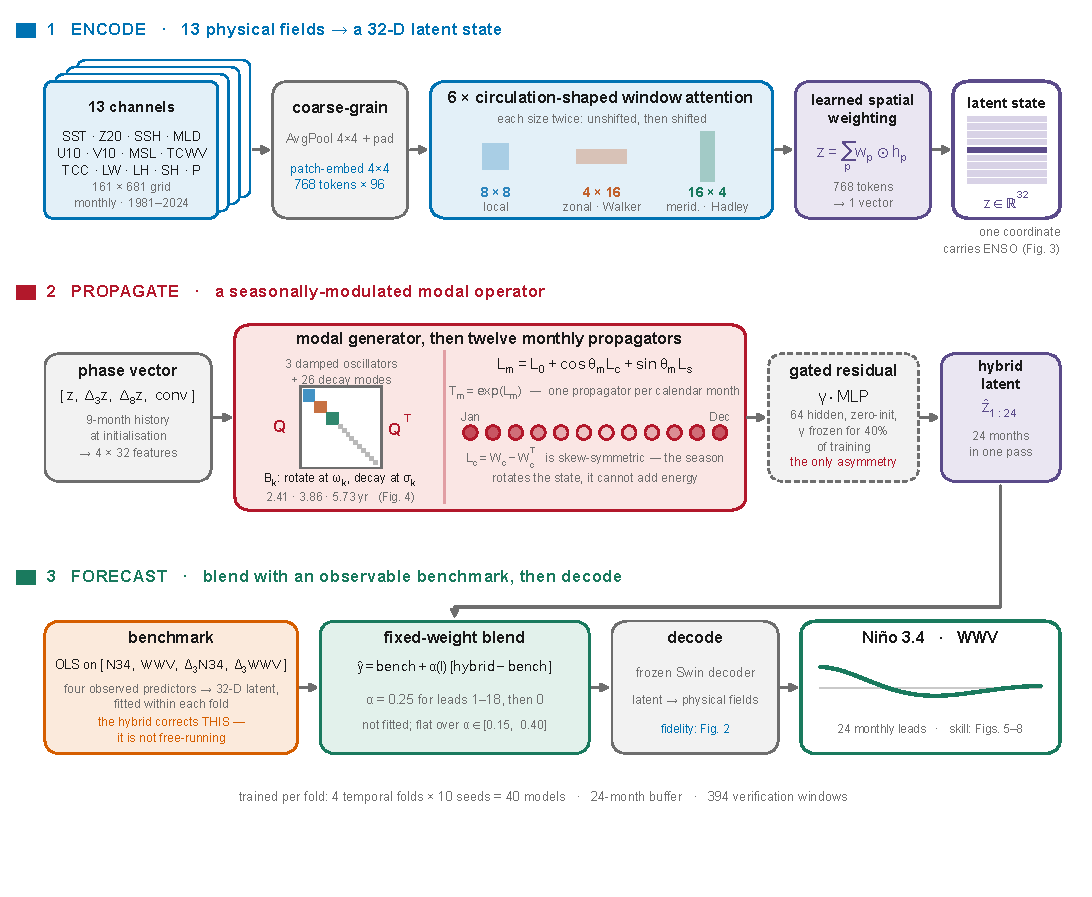
\includegraphics[width=\textwidth]{figures/fig01_schematic.pdf}
  \caption{The three stages of the forecast system. \textbf{(1) Encode.} Thirteen monthly
  physical fields on a $161\times681$ tropical-Pacific grid are coarse-grained and
  patch-embedded into 768 tokens, passed through six window-attention blocks whose windows are
  shaped to match the tropical circulation, and reduced by a learned spatial weighting to a
  32-dimensional state $z$. \textbf{(2) Propagate.} A phase vector built from a 9-month history
  drives a modal generator $L_0$ containing three damped oscillators and 26 decay modes; a
  Floquet seasonal modulation produces one propagator per calendar month; a $\gamma$-gated MLP
  supplies the shown nonlinear correction (three further terms present in every trained model
  -- a learned correction to the initial state, a state-dependent gain, and a low-rank direct
  linear term -- are omitted here for legibility and given in Sec.~\ref{sec:operator}).
  \textbf{(3) Forecast.} The hybrid latent trajectory is blended
  with an observable-predictor benchmark at fixed weight $\alpha=0.25$ out to lead 18, then
  decoded through the frozen Swin decoder to Ni\~no 3.4 and WWV over 24 monthly leads.}
  \label{fig:workflow}
\end{figure}
